\section{Background}
This section presents a brief history of traffic routing algorithms, defining the terminology
and the traffic routing problem.

\subsection{The Traffic Routing Problem}
Traffic routing problems naturally arise in communication or transportation networks, where users are trying to minimize the latency that they or their data experiences.
However, links in the network often becomes \emph{congested} if too many users decide to route their data 
or cars through that link. Consequently, in these networks, the path each user chooses can affect the travel times of other
users. Here, we describe Roughgarden and Tardos' formalization of the problem of minimizing latency as multicommodity flow networks~\cite{tardos,roughgarden}, and use Pigou's example network in Figure~\ref{fig:Pigou} as a running example. We use this to reason about the deviation from the opimum minimal latency when users make selfish routing decisions.

\begin{figure}[ht!]
\begin{center}
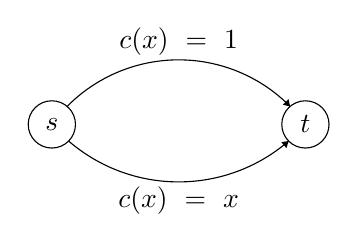
\begin{tikzpicture}[scale=0.1]
\tikzstyle{every node}+=[inner sep=0pt]
\draw [black] (18,-17.9) circle (3);
\draw (18,-17.9) node {$s$};
\draw [black] (50.2,-17.9) circle (3);
\draw (50.2,-17.9) node {$t$};
\draw [black] (19.94,-15.615) arc (135.3471:44.6529:19.905);
\fill [black] (48.26,-15.62) -- (48.05,-14.69) -- (47.34,-15.4);
\draw (34.1,-9.2) node [above] {$c(x)\mbox{ }=\mbox{ }1$};
\draw [black] (48.072,-20.011) arc (-49.23907:-130.76093:21.4);
\fill [black] (48.07,-20.01) -- (47.14,-20.15) -- (47.79,-20.91);
\draw (34.1,-25.7) node [below] {$c(x)\mbox{ }=\mbox{ }x$};
\end{tikzpicture}
\end{center}
    \caption{Pigou's example traffic routing problem, with a demand of $r_{(s,t)} = 1$}
\label{fig:Pigou}
\end{figure}

\medskip\noindent
\textbf{The input} to a traffic routing problem consists of:
\begin{itemize}
    \item A network $G = (V, E)$ of $|V|$ destinations (e.g., locations or servers) and $|E|$ links 
     \item A set of $k$ source-destination pairs $S=\{(s_1,t_1), \cdots (s_k,t_k)\}$ representing traffic demands
    \item A {rate} $r_i$ of traffic for each $(s_i,t_i)\in S$ representing the demanded amount of traffic from $s_i$ to $t_i$
    \item A {latency} cost function $c$ that assigns a per-edge function $c_e$ to each edge $e$ describing how adding traffic (i.e., congestion) to $e$ affects the time taken to travel across $e$. We can also think of $c$ as assigning per-path costs: for any path $p$ in the graph
        $$c_p(f) = \sum_{e\in P}c_e(f_e)$$ 
        We assume that $c$ is continuous, nonnegative, and nondecreasing.
\end{itemize}
In Figure~\ref{fig:Pigou}, we see a single source-destination input network with an example (linear) cost function with $r_{(s,t)} = 1$.

\medskip\noindent
\textbf{Solutions} correspond to flow assignments to the set of simple paths $P_i$ between $s_i$ and $t_i$ for all $i$.\footnote{Note that our solutions assume \emph{nonatomic} entities: the flows we find may not be integral. 
Intuitively, this means that the demand from one $s_i$ to $t_i$ is generated by an infinite number
of entities in the network, which allows us to reason about continuous, rather than discrete, functions.}
%
To describe a flow assignment $f$, we can consider $f_p$, the flow on a single path $p \in P_i$ (this adds an equal amount of flow $f_p$ to all edges in $p$), as well as $f_e = \sum_p \sum_{e\in p} f_p$, the flow on edge $e$ (the sum of flow on all paths that use $e$).

A \emph{feasible} solution given such an input is an assignment of path flows such that the demand from $s_i$ to $t_i$ is met:
$$\forall 1 \le i \le k,~\sum_{p\in P_i} f_p = r_i$$
%
An \emph{optimal} (feasible) solution given such an input is the feasible flow assignment $f$ that minimizes the \textbf{total weighted cost} $C(f)$, where
$$C(f) = \sum_i\sum_{p\in P_i}c_p(f)f_p = \sum_{e\in E} c_e(f_e)\cdot f_e$$
Intuitively, we are calculating the cost of each path of a given flow assignment, weighing 
each path's cost proportional to the amount of flow through the path. More concretely,
if we were to let flow represent the routes chosen by (infinitely many) users, $C(f)$ calculates the average cost over all users. Thus, when minimizing $C(f)$, some users may incur 
more latency so that other users can go faster: the optimal flow is the \emph{socially optimal} solution.
Note that there exists an optimal flow $f^*$ minimizing $C(f)$ because we assume $c$ is continuous and the set of feasible flows is compact.
We will also refer to the total weighted cost as the \textbf{social welfare} cost.

In our running example (Figure~\ref{fig:Pigou}), a feasible flow is any flow that sends one unit from $s$ to $t$ (divided in any fashion between the top and bottom edges).
The optimal flow is the flow that sends half the traffic through the lower edge and half through the upper edge: the users on the lower edge only experience a cost of $1/2$, while the users on the upper edge experience a cost of $1$, making the total weighted cost $3/4$.

\subsection{Coordination Models and the Price of Anarchy}
Before we can create algorithms to solve the traffic routing problem, we must first assume a \emph{coordination model} for our traffic network.
There are two clear extremes: (1) centralized control, in which some entity (e.g., an air traffic controller) knows all traffic demands and routes accordingly, and
(2) decentralization, i.e., a complete \emph{lack} of coordination between
entities in the network.
In a centralized setting, there is a clear optimal solution, as shown in the previous section.
However, in a decentralized and uncoordinated model, the lack of coordination and the exercise of freewill can result in
inefficiencies. 

\medskip
\textbf{The Price of Anarchy} (PoA) allows us to measure the inefficiencies of a decentralized model given some notion of equilibrium (how the flow assignment is determined in the model), and was first introduced by Koutsoupias and Papadimitriou in 1999~\cite{poa}. 
The PoA is defined as the ratio between the optimal flow and the flow achieved
at equilibrium.
(This is similar to how we measured the distance from optimal of an approximation algorithm in a limited computational power model, and of online algorithms in an incomplete information model.)

\subsection{The Selfish Routing Model}
One example of an uncoordinated model is the \emph{selfish routing} model, in which all entities in the network are selfish and choose a route minimizing their individual latency without caring (or knowing) about the effects on other users~\cite{tardos}.

The selfish routing model corresponds to flows at a \emph{Wardrop, or Nash equilibrium}~\cite{wardrop,haurie}.
The set of flows in a Nash equilibrium are defined such that for all $i$ source-destination pairs, all the paths from $s_i \to t_i$ have the minimum-possible cost. In other words, the (nonzero) 
flow paths at Nash equilibrium have equal path costs: 
$$\forall 0\le i \le k,~\forall p_1, p_2\in P_i~s.t.~f_{p_1} > 0~\text{and} f_{p_2} > 0,~ c_{p_1}(f) = c_{p_2}(f)$$

If we revisit our running example in Figure~\ref{fig:Pigou}, we note that the flow at Nash equilibrium corresponds to a flow that sends the entire unit of traffic through the bottom edge (the 0 flow through the top path has a cost of 1, and the unit flow through the bottom path will have cost 1).
Intuitively, each user routing from $s$ to $t$ will selfishly choose to take the bottom route because she will reason that the bottom route can have cost no worse than the top route. However, by doing so, the bottom route becomes more congested and leads to a total average cost $C(f) = 1$.
Thus, in Figure~\ref{fig:Pigou}, the price of anarchy $\rho$ is $\frac{1}{3/4} = \frac{4}{3}$.


\XXX{TODO should put more results about flows at Nash equilibrium? Not sure if important... the altruism paper has a good short description about how to compute Nash equilibria in polynomial time to 
find the selfish routing solution}

We next describe and present the main results regarding the PoA in this (decentralized) selfish routing model, which will act as a basis to which we will compare traffic routing results in more recently formulated models.

\subsection{Main Results}
\begin{theorem}
    If $f$ is a flow at Nash Equlibrium for a given input set $(G, r, c)$ and $f^*$ is a feasible flow for $(G, 2r, c)$, then $C(f) \leq C(f^*)$
\end{theorem}

\begin{proof-sketch}
    In other words, this result suggests that the latency when all users of a network route with only their own interests in mind is utmost the optimal (minimum) latency for the same graph and latency functions
    with twice as much demand per path. 
    
    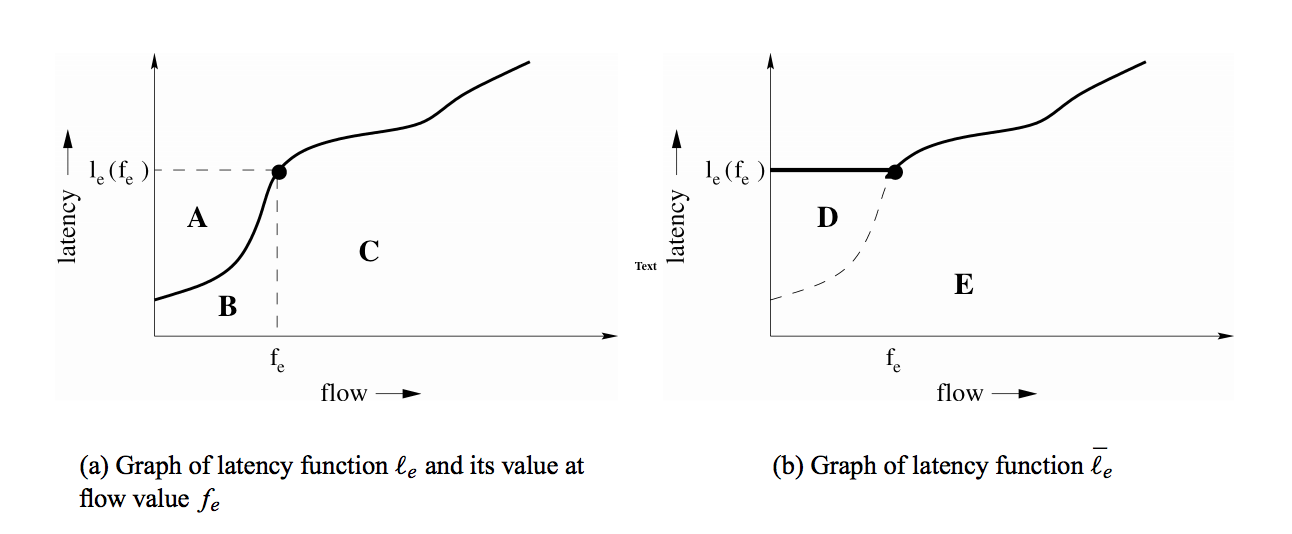
\includegraphics[width=1\textwidth]{graph}

    For any Nash Equilibrium solution $f$ for $(G, r, \ell)$ and any feasible solution $f^*$, we can draw the figures so that:
    
    The area under the black line from $0$ to $2f_e$ in subgraph (a) represents the cost of any feasible solution for $(G, 2r, \ell)$, and the area under the black line from $0$ to $2f_e$ in subgraph (b) represents the cost of any feasible solution for $(G, 2r, \ell)$. The area under the black line on the left side of $f_e$ in subgraph (a) represents the cost $C(f)$ of any Nash equilibrium solution for $(G, r, \ell)$. Note that since the area of t he area under the black line on the left side of $f_e$ in subgraph (a) is at least half of the dashed line, we know that the cost of any feasible solution for $(G, 2r, \ell)$, and the area under the black line from $0$ to $2f_e$ in subgraph (b) is at most $C(f)$ more than the cost of any feasible solution for $(G, 2r, \ell)$, and the area under the black line from $0$ to $2f_e$ in subgraph (a). So the area of the generalized trapezoid under the black line from $0$ to $2f_e$ is more than two times the area under the black line on the left side of $f_e$ in subgraph (b).
    
    The main idea of the proof for Theorem 1 lies in that the area under the black line between $f_e$ and $2f_e$ is at least as big as the area under the black line on the left side of $f_e$ in subgraph (b). This is always true because the latency $\bar{\ell}_e$ is a nondecreasing function and thus the graph of latency function gives a shape that looks like a generalized trapezoid (in particular, a right generalized trapezoid lying on the horizontal axis). Then we can obtain the result based on the property of a trapezoid shape. Therefore, the cost of any feasible solution for $(G, 2r, \ell)$ is at least twice the cost $C(f)$ of any Nash equilibrium solution for $(G, r, \ell)$. Then the area under the black line from $0$ to $2f_e$ in subgraph (a) is at least $2C(f)-C(f)$ and thus larger than $C(f)$. Therefore we have the result that the cost of any Nash equilibrium flow for $(G, r, \ell)$ is no bigger than represents the cost of any feasible solution for $(G, 2r, \ell)$.
    
\end{proof-sketch}

\begin{theorem}
    If the edge latency functions are linear in that $c_e = a_ef_e + b_e$ for every edge $e \in E$, then the price of anarchy or $\rho(G, R,l) \leq 4/3$.
\end{theorem}

\begin{proof-sketch}
    - describe some intuition for the $r/2$ case leading to $1/4$ cost of nash equilibrium
    - describe the augmentation that adds the $1/2$ factor.
\end{proof-sketch}
    
\XXX{TODO put results here}
\XXX{Result about unbounded PoA (use Pigou's example, maybe add figure)}
\XXX{Result about 4/3 PoA if functions linear}


